
% We first consider the value matrix $\bV:=[\bv(1),\cdots,\bv(N)]^\top \in \RR^{N \times D}$, and output matrix $\bU:=[\bu(1),\cdots,\bu(N)]^\top \in \RR^{N \times D}$ in self-attention as given by~(\ref{eqn:qkv}) and~(\ref{eq:attention-mat}), respectively, in Section~\ref{sec:background}. Let $\Omega \subset \RR$, $x \in \Omega$, and $\bv(x):=[v_{1}(x), \dots, v_{D}(x)]^T$ be a real vector-valued function, $\bv:\Omega \rightarrow \RR^{D}$, $\bv \in L^{2}(\Omega)$. Similarly, $\bu(x)$ be a real vector-valued function, $\bu:\Omega \rightarrow \RR^{D}$, $\bu \in L^{2}(\Omega)$ The value matrix $\bV$ and output matrix $\bU$ in self-attention discretizes the function $\bv(x)$ and $\bu(x)$ on a 1-D grid, respectively. In the context of control system, $\bv(x)$ can be considered as the state signal and $\bu(x)$ is the output signal of the following state-space model:


Consider the value matrix of layer ${\ell}$-th $\bV^{\ell}:=[\bv^{\ell}(1),\cdots,\bv^{\ell}(N)]^\top \in \RR^{N \times D}$ in Section~\ref{sec:background}. Let $\Omega \subset \RR$, $x \in \Omega$, and $\bv(x, t):=[v_{1}(x, t), \dots, v_{D}(x, t)]^T$ be a real vector-valued function, $\bv:\Omega \times [0, \infty)\rightarrow \RR^{D}$, $\bv \in L^{2}(\Omega \times [0, \infty))$. Assume the value matrix $\bV^{\ell}$ discretizes the function $\bv(x, t)$ on the spatial and time dimension. In the context of a control system, $\bv(x)$ can be considered as the state signal of the following state-space model:
\begin{align}
\label{eq:state-space}
\frac{d\bv(x, t)}{dt} &=\displaystyle \int_{\Omega}(\bv(y, t) - \bv(x, t))K(x, y, t)dy + \bz(x, t) \nonumber \\
    % \bm{u}(x, t) = \bv(x, t)\\
    \bv(x, 0) &= \bv^0(x), \bz(x, t) = \bm{0}, \forall x \in \Omega, \forall t \geq 0
\end{align}
where $\bm{z} \in L^{2}(\Omega \times [0, \infty))$ is a control input and $\bv^0$ is the initial state. 
%In our case, the output variable of the control system is the same as the state-variable $\bv$, hence, is discarded from~(\ref{eq:state-space}). 
The function $K(x, y, t)$ is the kernel function that captures the proximity of the signal $\bv$ at positions $x, y$ at time $t$.
Here, the SSM is autonomous, as no control inputs or feedback are fed into the system. In this section, we illustrate that system in~(\ref{eq:state-space}) induces smoothness to the signal by minimizing the nonlocal total variation~\cite{Gilboa2008NonlocalOW} of the signal, hence losing detailed information as it evolves. Subsequently, we show that self-attention serves as a discretization of this dynamic. Lastly, we theoretically demonstrate that the SSM in~\ref{eq:state-space} is vulnerable to input perturbation and representation collapse.

\vspace{-2mm}
\subsection{Connection between State Space Model and Nonlocal Variational Minimization}
\label{subsec:smooth-state-space}

We show that the gradient flow aimed at minimizing the following nonlocal functional is a case of our SSM described in~(\ref{eq:state-space})
\begin{equation}
    J(\bv) = \frac{1}{2} \int_{\Omega \times \Omega} \|\bv(x) - \bv(y)\|_2^2 k(x, y)dxdy.
\end{equation}
Here, $J(\bv)$, the sum of the square of the nonlocal derivative on the spatial dimension $\partial_y\bv(x) = \bigl(\bv(x) - \bv(y)\bigl)\sqrt{k(x,y)}$~\cite{Gilboa2008NonlocalOW}
, represents the non-local variation of the signal $\bv$. $k(x, y)$ captures the proximity between position $x$ and $y$ in the signal. Minimizing $J(\bv)$ promotes the smoothness of $\bv$ and penalizes high-frequency in the signal.

The gradient of $J$ with respect to $\bv$ is then given by
\begin{equation}
\begin{aligned}
\label{eqn:devJu}
    \nabla_{\bv} J(\bv) = \left[\frac{\partial J}{\partial v_1}, \frac{\partial J}{\partial v_2},  \dots, \frac{\partial J}{\partial v_{D}} \right]^T.
% \label{eq:}
\end{aligned}
\end{equation}
As shown in the Appendix~\ref{secapp:djv}, the Frechet derivative of $J$ with respect to $v_j$ is
\begin{align}  
\label{eq:partial-dev}
\frac{\partial J}{\partial v_j} 
&= \int_{\Omega}(v_j(x) - v_j(y)(k(x, y) + k(y, x))dy. 
\end{align}
Substituting the formula for ${\partial J}/{\partial v_j}$ in~(\ref{eq:partial-dev}) into~(\ref{eqn:devJu}) for $\nabla_{\bv} J(\bv)(x)$, we obtain the following gradient flow
\begin{equation}
\begin{aligned}
    \label{eq:gradient-descent}
    \frac{d\bv(x,t)}{dt} &= -\nabla_{\bm{v}}J(\bv) \\
    &= \int_{\Omega} \bigl(\bm{v}(y,t) - \bm{v}(x,t) \bigl)\bigl(k(x, y) + k(y,x)\bigl)dy,
\end{aligned}
\end{equation}
The autonomous state-space representation in~(\ref{eq:state-space}) simplifies to this dynamic when $K(x, y, t) := k(x, y) + k(y, x)$, which is symmetric and time-invariant. In this scenario, the model reduces the total nonlocal variance of the signal, resulting in a smoother solution. This renders the model susceptible to rank collapse in the output representation. In Section~\ref{subsec:state-space-analysis}, we prove that the model suffers from rank collapse regardless of whether $K(x, y, t)$ is symmetric.
% This property is crucial for enhancing   the model's robustness and reducing vulnerability to changes. 
% In Appendix~\ref{}, we will demonstrate that the smoothness of the solution persists even when we break the symmetry of the weighting function $K(x, y)$.

\textbf{Connection between SSM and self-attention.} We show that a discretization of our SSM recovers the self-attention mechanism. Let $\bq, \bk:\Omega \times [0, \infty) \rightarrow \RR^{D_{qk}}$, $\bq,\bk \in L^{2}(\Omega \times [0, \infty))$ be real vector-valued functions. Similar to $\bv(x, t)$, we can discretize $\bq(x, t),\bk(x, t)$ on spatial dimension to attain the query vectors $\bq^{\ell}(1), \dots, \bq^{\ell}(N) \in \RR^{D_{qk}}$, and the key vectors $\bk^{\ell}(1), \dots, \bk^{\ell}(N) \in \RR^{D_{qk}}$ of layer $\ell$-th. We define the proximity kernel as
\[
    K(x,y,t):= \frac{\exp\bigl(\bq(x, t)^{T}\bk(y, t)/\sqrt{D_{qk}}\bigl)}{\int_{\Omega}\exp\bigl(\bq(x, t)^{T}\bk(y', t)/\sqrt{D_{qk}}\bigl)dy'}.
\]
Applying the Euler method to discretize~(\ref{eq:state-space}) with the time step $\Delta t(x):= 1$, the update step of the system becomes
\begin{equation}
   \begin{aligned}
\label{eqn:sym-attn-cont}
&\bm{v}(x, t + 1) \\
\approx
&\displaystyle \int_{\Omega}\frac{\exp\bigl(\bq(x, t)^{T}\bk(y, t)/\sqrt{D_{qk}}\bigl)}{\int_{\Omega}\exp\bigl(\bq(x, t)^{T}\bk(y', t)/\sqrt{D_{qk}}\bigl)dy'} \bv(y, t)dy.
\end{aligned} 
\end{equation}

% \textbf{Self-attention as a discretization of the SSM.}
% Let $\bq(x, t):=[q_{1}(x, t), \dots, q_{D_{qk}}(x, t)]^T$, $\bk(x, t):=[k_{1}(x, t), \dots, k_{D_{qk}}(x, t)]^T$ be real vector-valued functions, $\bq, \bk:\Omega \times [0, \infty) \rightarrow \RR^{D_{qk}}$, $\bq,\bk \in L^{2}(\Omega, \times [0, \infty))$. Similar to $\bv(x, t)$, we can discretize $\bq(x, t),\bk(x, t)$ on spatial dimension to attain the query vectors $\bq^{\ell}(1), \dots, \bq^{\ell}(N) \in \RR^{D_{qk}}$, and the key vectors $\bk^{\ell}(1), \dots, \bk^{\ell}(N) \in \RR^{D_{qk}}$ of layer $\ell$-th.
% Using the Euler method to discretize~(\ref{eq:state-space}), with $\Delta t(x):= 1$, $K(x,y,t):= \displaystyle\frac{\exp\bigl(\bq(x, t)^{T}\bk(y, t)/\sqrt{D_{qk}}\bigl)}{\int_{\Omega}\exp\bigl(\bq(x, t)^{T}\bk(y', t)/\sqrt{D_{qk}}\bigl)dy'}$ the update step of the system becomes
% \begin{equation}
%    \begin{aligned}
% \label{eqn:sym-attn-cont}
% &\bm{v}(x, t + 1) \\
% \approx
% &\displaystyle \int_{\Omega}\frac{\exp\bigl(\bq(x, t)^{T}\bk(y, t)/\sqrt{D_{qk}}\bigl)}{\int_{\Omega}\exp\bigl(\bq(x, t)^{T}\bk(y', t)/\sqrt{D_{qk}}\bigl)dy'} \bv(y, t)dy.
% \end{aligned} 
% \end{equation}
Using the Monte-Carlo method~\cite{13ab5b5e-0237-33fb-a7a8-6f6e4e0d4e0f} to approximate the integrals in the spatial dimension in~(\ref{eqn:sym-attn-cont}), we attain 
\begin{equation}
\nonumber
\bm{v}^{\ell + 1}(i) \approx \sum_{j=1}^N{\rm softmax}\Big({\bq}^{\ell}(i)^\top{\bk}^{\ell}(j)/\sqrt{D_{qk}}\Big){\bv}^{\ell}(j).
\end{equation}
% \vspace{-0.1in}
which recovers $\bu^{\ell}(i)$, the output token $i$ of self-attention at layer $\ell$-th as in~(\ref{eq:attention-vec}). As self-attention discretizes the SSM outlined in~(\ref{eq:state-space}), it inherits the characteristics of the model, making it susceptible to input corruption and output rank collapse. These properties are theoretically demonstrated in Section~\ref{subsec:state-space-analysis}.
% \label{eqn:sym-attn-disr-2}

\vspace{-2mm}
\subsection{Stability and Representation Collapse of the State Space Model}
Model robustness is its ability to maintain high performance despite encountering uncertain or challenging scenarios such as noisy data, distribution shifts, or adversarial attacks~\cite{wang-bansal-2018-robust,dong2020benchmarking}.
Robustness also entails stability, wherein the model's output remains relatively unchanged even when the input is perturbed.

\label{subsec:state-space-analysis}
For the theoretical analysis of our SSMs, we assume that the kernel $K$ is time-invariant, i.e.,
$K(x,y,t)=K(x,y)$. This assumption is practical in the context of transformers, particularly in deep transformer models, where the attention matrix tends to remain similar after the initial layers~\cite{shi2022revisiting}.
The discretization of model in~(\ref{eq:state-space}) on the spatial dimension gives
\begin{equation}
\nonumber
    \displaystyle \frac{d\bv(i, t)}{dt} =\displaystyle \sum_{j = 1}^N(\bv(j, t) - \bv(i, t))K(i, j), 
\end{equation}
for $i,j = 1, 2, \dots, N$
By choosing $K(i,j):= {\rm softmax}\bigl(\bq(i)^{T}\bk(j)/\sqrt{D_{qk}}\bigl)$, its corresponding matrix representation is obtained as
\begin{align}
\label{eq:ode1}
    \bV'(t){dt} = \bK\bV(t) - \bV(t), \bV(0) = \bV^0,
\end{align}
where $\bm{K}$ is a right-stochastic matrix with all positive entries. In the context of transformer, $\bm{K}$ is the attention matrix and $\bV = [\bv^0(1), \dots, \bv^0(N)]^T$ is the value matrix at the first layer.
Lemma~\ref{lem:state-space-sol} sheds light on the stability and representation collapse of the solution for the SSM in~(\ref{eq:state-space}).
\begin{lemma}
    \label{lem:state-space-sol}
    Given $\{\alpha_1, \alpha_2,\dots, \alpha_M\}, M \leq N$, is the complex spectrum of $\bK - \bI \in \mathbb{R}^{N \times N}$. The solution of the ordinary differential equation (ODE)~(\ref{eq:ode1}) is given by
    \begin{align}
    \label{eq:state-space-sol}
        \bV(t) = \bm{P}\mathrm{exp}(\bm{J}t)\bm{P}^{-1}\bV^0,
    \end{align}
where $\bm{P}\bm{J}\bm{P}^{-1}$ is the Jordan decomposition of $\bm{K} - \bm{I}$, $\bm{P}$ is invertible and contains the generalized eigenvectors of $\bm{K} - \bm{I}$, and $\bm{J} = \bm{\mathrm{diag}}(\bm{J}_{\alpha_1, m_1}, \bm{J}_{\alpha_2, m_2}, \dots, \bm{J}_{\alpha_M, m_M}) $ is the Jordan form of matrix $\bm{K} - \bm{I}$ with,\\
$\bm{J}_{\alpha_i, m_i} = \begin{bmatrix} 
    \alpha_i &  1& \dots &0\\
   \vdots & \ddots & & \vdots\\
    &  & \alpha_i& 1\\
    0 & \dots    &   & \alpha_i
    \end{bmatrix} \in \mathbb{R}^{m_i \times m_i}$, for $i = 1, \dots, M$ are Jordan blocks. Here, $\sum_{i = 1}^Mm_i = N$.
\end{lemma}

The proof of Lemma~\ref{lem:state-space-sol} is shown in the Appendix~\ref{secapp:state-space-sol}. Since $\bK$ is a positive right-stochastic matrix, its largest and unique eigenvalue $\alpha_1$ is 1 and $|\alpha_i| < 1$ (see Theorem 4.1 in~\cite{strohmer2020mathdl}), meaning $\mathrm{Re(\alpha_i)} \in [-1, 1)$, for $i = 2, \dots, M$. Hence, the matrix $\bK - \bI$, whose eigenvalues are $\alpha_1 - 1, \dots, \alpha_M - 1$, has a unique largest eigenvalue of 0 and the real part of other eigenvalues in $[-2, 0)$. This leads to the rank collapse of the steady-state solution, as stated in the following Lemma~\ref{lem:steady-state-state-space-sol}.
\begin{lemma}
\label{lem:steady-state-state-space-sol}
     $\lim_{t \to \infty}\bV(t) = \begin{bmatrix} \displaystyle c_{1,1}\bm{p_1}, & \dots,&c_{1, D_x}\bm{p_1} \end{bmatrix}$,
    % $t \rightarrow \infty$ the solution in~(\ref{eq:state-space-sol}) will converge to $\begin{bmatrix} \displaystyle c_{1,1}\bm{p_1} & \dots & \displaystyle c_{1, D_x}\bm{p_1} \end{bmatrix}$, 
    where $\bm{p}_1$ is the eigenvector corresponds with the eigenvalue $(\alpha_1 - 1) = 0$ of $\bm{K} - \bm{I}$, and $c_{1,1}, \dots, c_{1,D_x}$ are the coefficients w.r.t $\bm{p}_1$ of the decomposition of $\bm{V}^0$'s columns in the Jordan basis (column vectors of $\bm{P}$).
\end{lemma}

\vspace{-2mm}
The proof of Lemma~\ref{lem:steady-state-state-space-sol} is shown in the Appendix~\ref{secapp:steady-state-state-space-sol}.
This yields two insights. Firstly, the steady-state solution of the system depends on the initial $\bm{V}^0$, implying that any perturbation in the input results in changes in the output. 
Secondly, the solution experiences rank collapse, with the rank of its steady state solution being 1 as $t \to \infty$. This indicates that our SSM in (\ref{eq:state-space}) not only yields a non-robust solution but also experiences information loss (low-rank output representation). As the self-attention mechanism discretizes the model in (\ref{eq:state-space}), it inherently exhibits both issues.
\vspace{-3mm}
\section{Transformer with PID-Controller for State-Space Representation}
\label{sec:pid-control}
To counteract the loss of detailed information caused by smoothness and to bolster model stability, a PID controller is integrated into the state-space representation as follows:
\begin{align}
\label{eq:state-space-pid}
    \displaystyle \frac{d\bv(x, t)}{dt} &=\displaystyle \int_{\Omega}(\bv(y, t) - \bv(x, t))K(x, y, t)dy + \bm{z}(x, t) \nonumber \\
    \bm{z}(x, t) &=\displaystyle \lambda_P\bm{e}(x, t) + \lambda_I\int_0^{t}\bm{e}(x, t) + \lambda_D\frac{d\bm{e}(x, t)}{dt} \nonumber \\
    \bv(x, 0) &= \bv^0(x), \bz(x, 0) = \bm{0}.
\end{align}

The regularizer term, denoted as $\bm{e}(x, t) = \bff(x) - \bv(x, t)$, encapsulates the loss of information as $\bv(x, t)$ becomes smoother over time. Here, the reference function $\bff(x)$ represents a high-frequency signal containing detailed information about the original inputs. We select $\bff(x)$ as the scaled initial value function, denoted as $\beta\bv(x, 0)$. In the context of a transformer, we set $\bff(i) = \beta\bv^0(i)$, representing the value vector embedding at token index $i$ of the first layer. This choice is motivated by our desire to have flexibility in determining the detailed information from the input signal we wish to preserve. This flexibility is governed by the parameter $\beta \in (0, 1]$. The regularizer $\bm{e}(x, t)$ is fed back into the system, guiding the model to reintegrate the lost information while maintaining stability through three components: (P), (I), and (D).

\vspace{-3mm}
\begin{itemize}
    \item The (P) term is directly proportional to the regularizer, $e(x, t)$. In cases of substantial information loss, the control input $\bz(x, t)$ should be proportionately large, determined by the gain factor $\lambda_P$, to reintroduce the lost information into the system. A small choice of $\lambda_P$ results in slow convergence, while a large choice may lead to overshooting issues, causing instability in reaching the reference point.
    \item The (I) term accumulates all past errors, given by $\lambda_I\int_0^{t}\bm{e}(x, t)$. This component aids in reintroducing any persistent, long-term loss of information that might persist despite proportional control.
    \item Finally, the (D) term, $\displaystyle \lambda_D\frac{d\bm{e}(x, t)}{dt}$, anticipates future losses of information by considering the rate at which the error is changing. A more rapid change in error prompts a greater control effect, and the derivative term proves beneficial in enhancing the stability and responsiveness of the control system.
\end{itemize}

\vspace{-3mm}
In this section, we unveil a connection between the two components, (P) and (I), of the SSM in~(\ref{eq:state-space-pid}) and different optimization methods applied to minimize a regularized functional. This functional is tailored to preserve the detailed information of the solution. Moreover, we show that the P-control (where $\lambda_I = \lambda_D = 0$), PD-control ($\lambda_I = 0$), and PID-controlled SSM in~(\ref{eq:state-space-pid}) are theoretically guaranteed to be more robust and mitigate the issue of rank collapse. Subsequently, we introduce the PID-controlled transformer (PIDformer), a novel architecture that enhances performance and robustness.

\vspace{-3mm}
\subsection{Connection between (P) and (I) Components with Different Optimization Methods} 

In Section~\ref{subsec:smooth-state-space}, we have shown that the SSM in~(\ref{eq:state-space}) implicitly performs a gradient descent to minimize the nonlocal variation $J(\bv)$, which leads to the loss of signal information. Now, we illustrate that the feedback-controlled state-space in~(\ref{eq:state-space-pid}), without the derivative (D) ($\lambda_D = 0$), implicitly minimizes the following functional:
\begin{equation}
  \begin{aligned}
    \label{eqn:energy-functional}
    E(\bv, \bff) &= J(\bv) + G(\bv,\bff) \\ 
    &= \frac{1}{2} \int_{\Omega \times \Omega} \|\bv(x) - \bv(y)\|_2^2 k(x, y)dx dy \\
    &+ \frac{\lambda}{2}  \int_{\Omega} \|\bv(x) - \bff(x)\|_2^2 dx.
    \end{aligned}  
\end{equation}
where the data fidelity term $G(\bv,\bff) = \frac{\lambda}{2} \int_{\Omega} \|\bv(x) - \bff(x)\|_2^2 dx$~\cite{Gilboa2008NonlocalOW, Gilboa2007NonlocalLI} is introduced to penalize significant information loss. This observation further validates that systems in~(\ref{eq:state-space-pid}) retains relevant information from the reference signal $\bff$.

\textbf{P-controlled SSM as gradient descent to minimize $E(\bv, \bff)$}.
The gradient of $E$ w.r.t $\bv$ is $\nabla_{\bv}E(\bv) = \nabla_{\bv}J(\bv) + \lambda \bigl(\bv(x) - \bff(x)\bigl)$.
The derivation of the derivative is given in Appendix~\ref{secapp:derE}.
Using the gradient descent method, we obtain the gradient flow:
\\
\begin{equation}
\label{eq:flowE}
    \begin{aligned}
        &\frac{d\bv(x,t)}{dt} = -\nabla_{\bm{u}}E(\bv) \\
        &= \int_{\Omega} \bigl(\bm{v}(y,t) - \bm{v}(x,t) \bigl)\bigl(k(x, y) + k(y,x)\bigl)dy \\
        &+ \lambda\bigl(\bff(x) - \bv(x, t)\bigl).
    \end{aligned}
\end{equation}
If we set
$K(x, y, t) := k(x, y) + k(y, x)$ to be symmetric and time-invariant, and $\lambda_P = \lambda, \lambda_I = \lambda_D = 0$, the controlled system in~(\ref{eq:state-space-pid}) simplifies to the gradient flow of $E$ in~(\ref{eq:flowE}). It suggests that integrating the (P) component into the system in~(\ref{eq:state-space}) minimizes the functional $E$ and reintroduces the lost information to the system.
% The gradient flow is a special case of our dynamic in~\ref{eq:state-space-pid} when we choose $\lambda_P = \lambda, \lambda_I = \lambda_D = 0$, which reduces to a P-controller.

\textbf{PI-controlled SSM as Bregman iteration to minimize $E(\bv, \bff)$}.
%
An alternative to gradient descent, Bregman iteration ~\cite{stanbregman,zhangnonlocalbregman} iteratively refines the solution by minimizing a Bregman divergence, which measures the discrepancy between the current solution and a reference point.
Given the convex functional $J(\bv)$, the Bregman divergence of $J$ between $\bv$ and $\bm{s} \in L^{2}(\Omega)$ is $D_J^p(\bv, \bm{s}) := J(\bv) - J(\bm{s}) - 
\langle  \bm{p} , \bv - \bm{s} \rangle $, where $\bm{p} \in \partial J(\bm{s})$, the subgradient of $J$ at $\bm{s}$. $D_J^p(\bv, \bm{s})$ captures the difference between $J(\bv)$ and the tangent plane $J(\bm{s}) - \langle\bm{p} , \bv - \bm{s}\rangle$.
The $\ell + 1$-th Bregman iteration to minimize $\min_{\bv}J(\bv)$ with the contraint $G(\bv, \bff)$ is given by:
\begin{align}\label{eqn:breg-op}
    \bv^{\ell + 1} &{=} \argmin_{\bv} D_J^{p^{\ell}}(\bv, \bv^{\ell}) + G(\bv, \bff), p^{\ell} \in \partial J(\bv^{\ell})
\end{align}

% To rewrite the optimization problem~\ref{eqn:breg-op} as the iteration of $\bv$ and $\bff$, we use the following lemma:
The following Lemma~\ref{lem:breg-iter} shows that the optimization problem in~(\ref{eqn:breg-op}) can be turned into solving iterative subproblems.
\begin{lemma}
\label{lem:breg-iter}
Applying Bregman iteration to minimize $E(\bv, \bff)$ involves solving iterative subproblems:
\begin{align} % cheat a little for the eq box to stay in the column
    \bv^{\ell + 1} &= \displaystyle \argmin_{\bv} J(\bv) + \frac{\lambda}{2} \int_{\Omega} \|\bv(x) - \bff(x) - \bm{e}^{\ell}_{\mathrm{a}}(x)\|_2^2 dx \nonumber \\
    \bm{e}^{\ell}_{\mathrm{a}}(x) &= \sum_{m = 1}^{\ell} \bm{e}^m(x) = \sum_{m = 1}^{\ell}\big( \bff(x) - \bv^m(x) \big),
%    & \bv^{\ell + 1} = \displaystyle \argmin_{\bv} J(\bv) + \frac{\lambda}{2} \int_{\Omega} \|\bv(x) - \bff^{\ell}(x)\|_2^2 dx \\
%  & \bff^{\ell}(x) = \bff^{\ell - 1}(x) + \bff(x) - \bv^{\ell}(x).
 \end{align}
\end{lemma}
The proof of Lemma~\ref{lem:breg-iter} is in Appendix~\ref{secapp:breg-iter}.
% The iteration in Lemma~\ref{lem:breg-iter} can be reformulated as:
% \begin{equation}
% \nonumber
%    \bv^{\ell + 1} = \displaystyle \argmin_{\bv} J(\bv) + \frac{\lambda}{2} \int_{\Omega} \|\bv(x) - \bff(x) - \bm{e}^{\ell}(x)\|_2^2 dx \\
% \end{equation}
Here, the term $\bm{e}^{\ell}_{\mathrm{a}}(x)$ captures the accumulated information loss between the original and the smoothed signals $\bv^m(x)$ of each iteration $m = 1, \dots, \ell$.
Taking a one-step update in the direction of gradient descent (see Appendix~\ref{secapp:grad-flow-breg}), we obtain
% the gradient flow at iteration $\ell + 1$ becomes
% \begin{equation}
% \begin{aligned}
%    \label{eq:grad-flow-breg}
%         \displaystyle\frac{d\bv(x, t)}{dt} &= \int_{\Omega} \bigl(\bm{v}(y,t) - \bm{v}(x,t) \bigl)\bigl(k(x, y) + k(y,x)\bigl)dy \\
%         &+ \lambda \bigl(\bff(x) - \bv(x, t) + \bm{e}^{\ell}(x)\bigl).
% \end{aligned}
% \end{equation}
% Appendix~\ref{secapp:grad-flow-breg} contains the derivation of the gradient flow in~(\ref{eq:grad-flow-breg}). Applying Euler method to discretize~(\ref{eq:grad-flow-breg}) with $\Delta t = 1$ and $\bv(x, 0) = \bv^{\ell}(x)$, we approximate the $\bv^{\ell + 1}$ with one-step gradient descent:
\begin{align}
   \label{eq:dis_breg}
   \bv^{\ell + 1}(x) 
   % \approx \bv(x, 1) 
   &= \int_{\Omega} \bigl(\bm{v}^{\ell}(y) - \bm{v}^{\ell}(x) \bigl)\bigl(k(x, y) + k(y,x)\bigl)dy \nonumber \\
   & + \bv^{\ell}(x) + \lambda \bm{e}^{\ell}(x) + \lambda\bm{e}^{\ell}_{\mathrm{a}}(x).
\end{align}
On the other hand, the Euler discretization with $\Delta t = 1$ of the PI-controlled state-space in~(\ref{eq:state-space-pid}) (as $\lambda_D = 0$) is:
\begin{equation}
\begin{aligned}
\label{eq:dis-PI}
    \bv^{\ell + 1}(x) &= \bv^{\ell}(x) + \int_{\Omega} \bigl(\bm{v}^{\ell}(y) - \bm{v}^{\ell}(x) \bigl)K(x, y)dy \\
    &+ \lambda_P \bm{e}^{\ell}(x) + \lambda_I \sum_{m = 1}^{\ell} \bm{e}^m(x).
\end{aligned}
\end{equation}
By selecting a time-independent $K(x, y, t) := k(x, y) + k(y, x)$ and setting $\lambda_P = \lambda_I = \lambda$, the update step of the PI-controlled model in~(\ref{eq:dis-PI}) simplifies to the update step of Bregman iteration in~(\ref{eq:dis_breg}). This connection suggests that the PI-controlled SSM minimizes $E(\bv, \bff)$.
\subsection{Stability and Representation Collapse of PID-Controlled State Space Model}

In this section, we aim to show that: (i) Integrating the (P) term enhances robustness against input perturbations and mitigates rank collapse of the output representation; (ii) Adding the (D) term in PD-control further stabilizes the system by mitigating rapid and unstable changes of $\bV(t)$, (iii) finally, integrating the (I) term in the PID-controlled SSM described in~(\ref{eq:state-space-pid}) guarantees system stability, making it robust to input corruption. Following the same assumption in Section~\ref{subsec:state-space-analysis}, we assume that $K(x, y, t)$ is time-invariant for our theoretical analysis in this section.
\subsubsection{Analysis of P-control SSM}
\label{subsec:PD-robust}
\textbf{Robustness of P-controlled SSM.}
From the SSM in~(\ref{eq:state-space-pid}), by choosing $\lambda_I = \lambda_D = 0$, and applying Euler discretization on the spatial domain, the P-control model is given as:
%%%%%% TAM: change this state-space to the original P-control
\begin{equation}
   \begin{aligned}
\label{eq:state-space-P}
% \nonumber
    \displaystyle \frac{d\bv(i, t)}{dt} &=\displaystyle \sum_{j = 1}^N(\bv(j, t) - \bv(i, t))K(i, j) \\
    &+ \lambda_P \bigl(\bff(i) -  \bv(i, t)\bigl), 
\end{aligned} 
\end{equation}
for $i,j = 1, 2, \dots, N$, and $K(i,j):= {\rm softmax}\bigl(\bq(i)^{T}\bk(j)/\sqrt{D_{qk}}\bigl)$. The corresponding matrix representation is given as
\begin{equation}
\begin{aligned}
    \label{eq:odeP}
    \frac{d\bV(t)}{dt} = \bK\bV(t) - (\lambda_P + 1)\bV(t) + \lambda_P \bm{F}, \bV(0) = \bV^0.
\end{aligned}
\end{equation}
where $\bm{F} = [ \bff(1), \dots, \bff(N) ]^T$.
The following Lemma~\ref{lem:state-space-P-sol} help us analyze the stability and representation collapse of the solution for the SSM in~(\ref{eq:odeP}).
% To simplify our analysis, we assume that $\bK - (\lambda_P + 1)\bI$ is invertible. 
Here, since the eigenvalues of $\bK$ the has the real part in $[0, 1]$, $\lambda_P + 1$ ($\lambda_P > 0$) can not be one of them. This implies that $\mathrm{det}(K - (\lambda_P + 1)I) \neq 0$ hence the matrix is non-singular.
% TAM note: (The proof of the lemma doesnt depends on the invertibility of B, but i show that B is invertible nonetheless for simplification in notation).
\begin{lemma}
    \label{lem:state-space-P-sol}
    Let $\bm{B} := \bK - (\lambda_P + 1)\bI \in \mathbb{R}^{N \times N}$, the solution of the ordinary differential equation~(\ref{eq:odeP}) is
    \begin{align}
    \label{eq:state-space-P-sol}
    \bV(t) = \mathrm{exp}(\bm{B}t)(\bV^0 + \bm{B}^{-1}\bm{F}) - \lambda_P\bm{B}^{-1}\bm{F}.
        % \bV(t) =  \begin{bmatrix} \displaystyle \sum_{i}^{N}c_{i,1}e^{\alpha_it}\bm{r}_i - \lambda_P\bm{B}^{-1}\bm{F}_{., 1}& \dots & \displaystyle \sum_{i}^{N}c_{i,D_x}e^{\alpha_it}\bm{r}_i - \lambda_P\bm{B}^{-1}\bm{F}_{., D_x}\end{bmatrix}.
    \end{align} If $\bm{B}$ has only eigenvalues with negative real parts, then $\lim_{t \to \infty}\bm{V}(t) = -\lambda_P\bm{B}^{-1}\bm{F}$.
\end{lemma}
The proof of Lemma~\ref{lem:state-space-P-sol} is shown in the Appendix~\ref{secapp:state-space-P-sol}. As shown in Section~\ref{subsec:state-space-analysis}, since the eigenvalues of $\bm{K}$ has $\mathrm{Re}(\alpha_i) \in [-1, 1], i = 1, \dots, M$, therefore the real parts of eigenvalues of $\bm{B}$ must be in the range $[-2 - \lambda_P, -\lambda_p]$, which are all negative. As the result of~\ref{lem:state-space-P-sol}, the steady state solution in~(\ref{eq:state-space-P-sol}) $\lim_{t \to \infty}\bm{V}(t) = -\lambda_P\bm{B}^{-1}\bm{F}$. Therefore, adding any perturbation to the initial state $\bV^0$ does not change the steady state solution. However, in our context of a transformer, the perturbation also affects the reference point $\bm{F}$, which is chosen to be a scaled $\beta\bm{\bV}^0$, leading to the steady state solution becomes $-\lambda_P\beta\bm{B}^{-1}\bm{\bV}^0$. Fortunately, the P-control system allows the error caused by perturbation to be as neglectable as desired. The following Proposition~\ref{lem:lambda_P} confirms the robustness of the P-control SSM.
%%%%%% TAM: explain why choosing the scaled v^0: ablation study
\begin{proposition}
\label{lem:lambda_P}
    Given the coefficient $\lambda_P > 0$ in~(\ref{eq:state-space-pid}), and any arbitrary $\Bar{\epsilon}, \delta > 0$, by adding  the perturbation $\bm{\epsilon} \in \mathbb{R}^{N \times D}, \| \bm{\epsilon} \|_{\infty} \leq \Bar{\epsilon}$ to $\bV^0$, the corresponding change in the steady state solution of the system in~(\ref{eq:odeP}) is independent of $\lambda_P$ and becomes negligible with an amount of at most $\delta$ if 
    \begin{align}
        \beta \leq {\delta}/{\bar{\epsilon}}.
    \end{align}
\end{proposition}
%%%%%% TAM: giving the insights why the change doesnt depend on lamda_p
\vspace{-2mm}
The proof of Proposition~\ref{lem:lambda_P} is shown in the Appendix~\ref{secapp:lambda_P}.
Proposition~\ref{lem:lambda_P} suggests that we can select the hyper-parameter $\beta$ to make the impact of input perturbation on the output as small as desired.

\textbf{P-controlled SSM on representation collapse.} Since $\bm{B}^{-1}$ is full rank ($\bm{B}$ is non-singular), hence $\mathrm{rank}(-\lambda_P\bm{B}^{-1}\bm{F}) = \mathrm{rank}(\bm{F})$~\cite{strang2006linear}. In the case of a transformer, when choosing $\bm{F} = \beta \bV^0$, the rank of the steady state solution equals the rank of the input $\bV^0$. This implies that the P-control dynamic in~(\ref{eq:odeP}) prevents rank collapse.
% \begin{lemma}
%     \label{lem:rank-P}
%     If $\lambda_P + 1$ is different from all eigenvalues of $\bK$, then $\bm{B}$ is invertible and $-\lambda_P\bm{B}^-1\bm{F}$ is full rank.  
% \end{lemma}
% The proof of Lemma~\ref{lem:rank-P} is provided in Appendix~\ref{}. Lemma~\ref{lem:rank-P} suggests that we can always choose an positive $\lambda_P$  that prevents rank collapse of the steady state solution. Notice that, in practice, as $K$ is the attention matrix, it is easy to choose a random positive $\lambda_P$ that satisfies the above condition, without knowing the eigenvalues of $\bm{K}$, especially when the attention matrix is low-rank.
%%% put D in so that increase in stability, cuz lamda_d always > 0
\subsubsection{Analysis of PD-controlled SSM}
Since $\lambda_D \frac{d\bm{e}(x, t)}{dt} = \lambda_D \frac{d}{dt}(\bm{f}(x) - \bm{v}(x, t)) = -\lambda_D\frac{d\bm{v}(x, t)}{dt}$,
from the SSM in~(\ref{eq:state-space-pid}), by choosing $\lambda_I = 0$, $K(i,j):= {\rm softmax}\bigl(\bq(i)^{T}\bk(j)/\sqrt{D_{qk}}\bigl)$ for $i,j = 1, 2, \dots, N$, and applying Euler discretization on the spatial domain, the PD-control model can be represented in the matrix form:
\begin{equation}
\label{eq:odePD}
    \begin{aligned}
    \bV'(t) &= \bK\bV(t) - (\lambda_P + 1)\bV(t) + \lambda_P \bm{F} - \lambda_D\bV'(t)\\
    &= \frac{1}{1 + \lambda_D}\bigl(\bm{K} - (\lambda_P + 1)\bm{I}\bigl)\bV(t) + \frac{\lambda_P}{1 + \lambda_D}\bm{F},
\end{aligned}
\end{equation}
with $\bV(0) = \bV^0$.
The solution of~(\ref{eq:odePD}) is provided in the following Lemma~\ref{lem:state-space-PD-sol}.
\begin{lemma}
    \label{lem:state-space-PD-sol}
    Let $\bm{B} := \bK - (\lambda_P + 1)\bI \in \mathbb{R}^{N \times N}$, the solution of the ordinary differential equation~(\ref{eq:odePD}) is 
    \begin{align}
    \nonumber
    \label{eq:state-space-PD-sol}
    \bV(t) = \mathrm{exp}(\frac{1}{1 + \lambda_D}\bm{B}t)(\bV^0 + \bm{B}^{-1}\bm{F}) - \lambda_P\bm{B}^{-1}\bm{F}.
    \end{align} 
and $\lim_{t \to \infty}\bm{V}(t) = -\lambda_P\bm{B}^{-1}\bm{F}$.
\end{lemma}
The proof of Lemma~\ref{lem:state-space-PD-sol} is provided in Appendix~\ref{secapp:state-space-PD-sol}. This intriguing result suggests two key insights. Firstly, incorporating the (D) component into the P-control system does not alter the steady state of the solution. Consequently, the solution of the PD-controlled SSM retains the advantages of a P-control model, including avoiding rank collapse and ensuring bounded error. Secondly, the derivative term offers an additional benefit of further stabilizing the system by decreasing the eigenvalue by a factor of $\displaystyle{1}/({1 + \lambda_D})$, thereby mitigating rapid changes in $\bV(t)$.
% \begin{prop}
% \label{prop:pd-control-analysis}
% % TAM: rewrite this proposition
%      PD-control state space model in Eqn.~\ref{eq:odePD}  prevents rank collapse. Further more, given $\bm{F} = \beta\bV_0$, $\beta, \lambda_P, \lambda_D > 0$ are the coefficients of the (P) and (D) control terms, respectivaly, and if a bounded perturbation applied on the input $\bV^0 + \bm{E}, \bm{E} \leq \bar{\epsilon}$, then the change imposed on the solution of PD-control system in Eqn~\ref{eq:odePD}, as $t \rightarrow 0$ is made as arbitrarily small $\displaystyle \| \frac{-\lambda_P\beta}{1 + \lambda_D}\bm{B}^{-1}\bm{E}\|_{\infty} \leq \delta$ when $\displaystyle \frac{\beta}{\lambda_D + 1} < \frac{\delta}{\bar{\epsilon}}$. 
% \end{prop}
\subsubsection{Analysis of PID-controlled SSM}

Following the same analysis in Section~\ref{subsec:PD-robust}, by choosing $K(i,j):= {\rm softmax}\bigl(\bq(i)^{T}\bk(j)/\sqrt{D_{qk}}\bigl)$ and discretizing on the spatial domain, the matrix representation of the PID-controlled SSM reduced from~(\ref{eq:state-space-pid}) becomes
\begin{equation}
 \begin{aligned}
\label{eq:matrix-PI}
   \bV'(t) =&\frac{1}{\lambda_D + 1} \Bigg( \bigl(\bK - (\lambda_P + 1)\bm{I}\bigl)\bV(t) \\
   &+ \lambda_I \int_{0}^t (\bm{F} - \bV(t))dt
    + \lambda_P \bm{F} \Bigg),
\end{aligned}   
\end{equation}
where $\bV(0) = \bV^0$. To deal with the integral in~(\ref{eq:matrix-PI}), we take the derivative of both sides, the equation becomes $\bV''(t) = \displaystyle \frac{1}{\lambda_D + 1} \big(\big(\bK - (\lambda_P + 1)I \big)\bV'(t) - \lambda_I\bV(t) \big)$, which is turned into a system of 1-st order differential equation:
\begin{equation}
\begin{aligned}
    \label{eq:ode-pi}
    \begin{bmatrix} \bV'(t) \\ \bV''(t) \end{bmatrix} &= \begin{bmatrix} \bm{0} & \bm{I} \\ \displaystyle -\frac{\lambda_I\bm{I}}{\lambda_D + 1} &\displaystyle \frac{\bm{K} - (\lambda_P + 1)\bm{I}}{\lambda_D + 1} \end{bmatrix} \begin{bmatrix} \bV(t) \\ \bV'(t) \end{bmatrix},
    % &=: \bm{M}\begin{bmatrix} \bV(t) \\ \bV'(t) \end{bmatrix} , 
\end{aligned}
\end{equation}
where $\bV(0) = \bV^0$, and $\bV'(0) =\displaystyle \frac{1}{\lambda_D + 1} \big( (\bm{K} - (\lambda_P + 1))\bV^0 + \lambda_P\bm{F} \big)$.
To gain robustness, the steady state solution of the model should be independent of any perturbation of the input $\bV_0$
% , requires the eigenvalues $\bm{M}$ to have negative real part (see Appendix~\ref{secapp:first-order-ode}). 
The following Proposition~\ref{lem:lambda_PI} illustrates the stability of the system.
%%% lamda_i too big make it unstable
\begin{proposition}
    \label{lem:lambda_PI} For any $\lambda_P, 
    \lambda_I, \lambda_D > 0$, the system in~(\ref{eq:ode-pi}) has a stable solution.
\end{proposition}
The proof of Proposition~\ref{lem:lambda_PI} is in the Appendix~\ref{secapp:lambda_PI}. 
The Proposition implies that the PID-controlled SSM in~(\ref{eq:state-space-pid}) remains robust and stable for any selection of positive values for $\lambda_P, \lambda_I, \lambda_D$.
% \textbf{On the representation collapse of PID-control state-space system}

\subsection{Transformer with PID Control}
By applying the Euler discretization with time step $\Delta t = 1$, initializing $\bv$ at $t = 0$ as $\bv(x, 0) = v^0(x)$, and choosing 
\[
K(x,y, t):= \frac{\exp\bigl(\bq(x, t)^{T}\bk(y, t)/\sqrt{D_{qk}}\bigl)}{\int_{\Omega}\exp\bigl(\bq(x, t)^{T}\bk(y', t)/\sqrt{D_{qk}}\bigl)dy'},
\]
the update step of PID-controlled SSM in~(\ref{eq:state-space-pid}) becomes:
\begin{equation}
  \begin{aligned}
\label{eq:pid-dis-t}
    &\bv^{\ell + 1}(x) \\
    &\approx  \int_{\Omega} \bigl(\bm{v}^{\ell}(y) - \bm{v}^{\ell}(x) \bigl)\displaystyle\frac{\exp\bigl(\bq^{\ell}(x)^{T}\bk^{\ell}(y)/\sqrt{D_{qk}}\bigl)}{\int_{\Omega}\exp\bigl(\bq^{\ell}(x)^{T}\bk^{\ell}(y')/\sqrt{D_{qk}}\bigl)dy'}dy \\
    &+ \bv^{\ell}(x) + \lambda_P \bm{e}^{\ell}(x) + \lambda_I \sum_{m = 1}^{\ell} \bm{e}^m(x) + \lambda_D(\bm{e}^{\ell}(x) - \bm{e}^{\ell - 1}(x)),
\end{aligned}  
\end{equation}
where $\bm{e}^m(x) = \bff(x) - \bv^m(x)$ for $m = 1,\dots, \ell$. 
Applying the Monte-Carlo method to approximate the integrals in~(\ref{eq:pid-dis-t}) and discretizing $\bv^{l + 1}(x)$, $\bv^m(x)$, and $\bv_0(x)$ on a spatial dimension, and by choosing $\bff(x) = \bv(x)$, we attain the output of the following novel PID-attention at layer $\ell$-th is defined as
\begin{definition}[PID-control Transformer (PIDformer)]
\label{def:pid-attn}
Given a set of key and value vectors $\{\bk^{\ell}(j),\bv^{\ell}(j)\}_{j=1}^{N}$ in each layer $\ell$, $\ell=1,\dots,L$, for each query vector $\bq^{\ell}(i)$, $i=1,\dots,N$, in the same layer, the self-attention unit at layer $\ell$ in a PID-control Transformer (PIDformer) computes the corresponding output vector $\bu^{\ell}(i)$ of the query $\bq^{\ell}(i)$ by the following attention formula:
\begin{equation}
   \begin{aligned}
    \bu^{\ell}(i)  
    &=\sum_{j = 1}^N {\rm softmax}\Big({\bq}^{\ell}(i)^\top{\bk}^{\ell}(j)/\sqrt{D_{qk}}\Big)\bm{v}^{\ell}(y) \\
    &+ \lambda_P \bm{e}^{\ell}(i) + \lambda_I \sum_{m = 1}^{\ell} \bm{e}^{m}(i) + \lambda_D(\bm{e}^{\ell}(i) - \bm{e}^{\ell - 1}(i)),
\end{aligned} 
\end{equation}
where $\bm{e}^{\ell} = \bv^0 - \bv^{\ell}$, $\bv^{0}(1),\dots, \bv^{0}(N)\in \RR^{D}$ are the value vectors in the first layer of PIDformer. 
\end{definition}
Since PID-attention is a discretization of the controlled SSM in (\ref{eq:state-space-pid}), it is inherently a more robust attention mechanism.
Fig.~\ref{fig:pid-illustrate} illustrates the architecture of PIDformer.

\begin{figure}[!t]
\centering
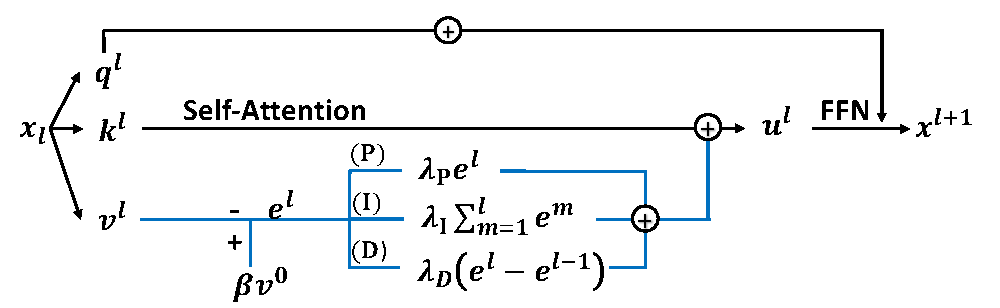
\includegraphics[width=0.48\textwidth]{iclr_2023/pictures/pid.pdf}
\vspace{-0.3in}
\caption{\small Our proposed PIDformer model at each layer.}
\label{fig:pid-illustrate} 
% \vspace{-0.in}
\end{figure}